%%%%%%%%%%%%%%%%%%%%%%%%%%%%%%%%%%%%%%%%%%%%%%%%%%%%%%%%%%%%%%%%%%%%%%%%%%%%%%%%
%2345678901234567890123456789012345678901234567890123456789012345678901234567890
%        1         2         3         4         5         6         7         8

\documentclass[letterpaper, 10 pt, conference]{ieeeconf}  % Comment this line out if you need a4paper

%\documentclass[a4paper, 10pt, conference]{ieeeconf}      % Use this line for a4 paper

\IEEEoverridecommandlockouts                              % This command is only needed if 
                                                          % you want to use the \thanks command

\overrideIEEEmargins                                      % Needed to meet printer requirements.

%In case you encounter the following error:
%Error 1010 The PDF file may be corrupt (unable to open PDF file) OR
%Error 1000 An error occurred while parsing a contents stream. Unable to analyze the PDF file.
%This is a known problem with pdfLaTeX conversion filter. The file cannot be opened with acrobat reader
%Please use one of the alternatives below to circumvent this error by uncommenting one or the other
%\pdfobjcompresslevel=0
%\pdfminorversion=4

% See the \addtolength command later in the file to balance the column lengths
% on the last page of the document

\usepackage{graphics} % for pdf, bitmapped graphics files
\usepackage{epsfig} % for postscript graphics files
\usepackage{mathptmx} % assumes new font selection scheme installed
\usepackage{times} % assumes new font selection scheme installed
\usepackage{amsmath} % assumes amsmath package installed
\usepackage{amssymb}  % assumes amsmath package installed
%\usepackage{amsthm}
\usepackage{bm}
\usepackage{mathrsfs}
\usepackage{color}
\usepackage{cite}
\usepackage{threeparttable}

\usepackage{multirow}
\usepackage{bigdelim}

\usepackage{algorithm}
\usepackage{algorithmicx}
\usepackage{algpseudocode}

\usepackage{graphicx}
\usepackage{subfigure}

\usepackage{url}

%\usepackage[all]{xy}

\newtheorem{theorem}{Theorem}[section]
\newtheorem{definition}{Definition}[section]
\newtheorem{lemma}{Lemma}[section]
\newtheorem{remark}{Remark}[section]
\newtheorem{corollary}{Corollary}[section]
\newtheorem{notation}{Notation}[section]
\newtheorem{problem}{Problem}[section]

\floatname{algorithm}{Algorithm}
\renewcommand{\algorithmicrequire}{\textbf{Input:}}
\renewcommand{\algorithmicensure}{\textbf{Output:}}

\title{\LARGE \bf
Optimal Task-Space Tracking with Minimum Manipulator Reconfiguration
}


\author{Tong Yang$^{1}$~\IEEEmembership{Student Member,~IEEE}, Jaime Valls Miro$^2$~\IEEEmembership{Member,~IEEE}, \\Yue Wang$^{1*}$~\IEEEmembership{Member,~IEEE} and Rong Xiong$^1$~\IEEEmembership{Member,~IEEE}
\thanks{$^1$ Tong Yang, Yue Wang and Rong Xiong are with the State Key 
Laboratory of Industrial Control and Technology, Zhejiang University, P.R. China. 
}
\thanks{$^2$ Jaime Valls Miro is with the Robotis Institue at the University of Technology Sydney (UTS:RI), Sydney, Australia.}
\thanks{This work was partially supported by National Key R\&D Program of China (2018AAA0102700), and in part by the Science and Technology project of Zhejiang Province (Grant No.2019C01043).}
\thanks{$^*$ Corresponding author: {\tt\small wangyue@iipc.zju.edu.cn}}
}


\begin{document}

\maketitle
\thispagestyle{empty}
\pagestyle{empty}

%%%%%%%%%%%%%%%%%%%%%%%%%%%%%%%%%%%%%%%%%%%%%%%%%%%%%%%%%%%%%%%%%%%%%%%%%%%%%%%%
\begin{abstract}
An optimal solution to the task-space tracking problem using a non-redundant manipulator is proposed. This is a recurring occurrence in automated manufacturing settings, 
e.g.  welding, deburring, painting, %quality control of a finished part, 
%close inspection along a crack on a surface etc.
or quality control inspections. 
Given a pre-defined %task-space 
path for the end-effector to follow, there may not exist a joint-space continuous solution for task-space tracking when the non-linear manipulator kinematics and collision avoidance with obstacles in the workcell are considered. This introduces undesirable manipulator reconfigurations where the end-effector is required to deviate temporarily from the pre-defined path. 
The unwanted motion results in pausing task-space tracking, incurring not only ineffective time and energy demands but potentially compromising the quality of the task at hand due to the additional discontinuities. 
%(e.g. welding or painting). 
%Moreover, it also imposes the need for larger obstacle-free workcell operating environment to accomodate for the manipulator reconfiguration.% <JVM> this is true, yet since we don't 'remove' the discontinuity, this undesirable effect remains even if we have to do it only once. Abstract is quite long, so I have axed. I will see if it can be added elsewhere
An algorithm is proposed that provides a globally optimal perspective to the choice of suitable joint-space connected segments so that the minimum number of manipulator reconfigurations during task-space tracking is guaranteed.  By carefully selecting the inverse kinematic solutions, all sequences %of invese kinematics solutions 
ensuring minimum reconfigurability are proven collected by  Dynamic Programming. 
%generalises the problem to 
%The algorithm proposed in this work globally solves the task-space tracking problem. 
Moreover, a faster greedy strategy is suggested to increase the computational efficiency of the tracker whilst still preserving global optimality and completeness. 
% <JVM> Not sure completeness is proven, pls confirm, then we can 
% real-time solvable in a dynamic programming scheme. % <JVM> we don't show in numbers the speed-up that we claim, this is a bit flimsy. Ideally we would perhaps have to compare with full DP to show the speed-up. In that regard, "real-time" is not really proven, and we should not claim it. It is the kind of thing that reviewers seasoned in path planning will aim for to shoot the work down, path planning has been researched very extensively, there will be many reviewers with this background out there ...
The effectiveness of the proposed algorithm is validated against traditional sampling-based solvers in simulation and illustrated on challenging real-world tracking experimentation with a Universal Robotics manipulator and a curved-surface object, depicted also in an accompanying video. 
An open-source implementation has also been provided for the benefit of the robotics community. 
\end{abstract}

%%%%%%%%%%%%%%%%%%%%%%%%%%%%%%%%%%%%%%%%%%%%%%%%%%%%%%%%%%%%%%%%%%%%%%%%%%%%%%%%
\section{Introduction}
The task-space non-revisiting tracking problem (TNTP) of a manipulator~\cite{Liang2010Adaptive} is a fundamental module that appears often in real-world applications, e.g.  welding~\cite{Norberto2003Welding}, inspection~\cite{Nakhaeinia2013Trajectory}~\cite{Simetti2016Underwater} or other general maintenance duties~\cite{Simetti2016Underwater}. 
In these applications, the task-space path for a manipulator equipped with the appropriate tool is generally pre-defined~\cite{Chen2019Synchronization}, and the problem is to generate a valid manipulator joint-space trajectory ensuring the end-effector (EE)  visits each point on the task-space path in order, and exactly one time~\cite{Janiak2017Motion}. 
However, a continuous singularity-free joint-space trajectory %holding the EE on the task-space waypoints 
may be impeded by the manipulator kinematic constraints, and the motion made even more restricted by the obstacles present in the environment. As such the manipulator may be forced to undertake joint-space reconfigurations resulting in the EE departing from the pre-assigned path. 
%Between the EE leaving and re-touching the task-space path, the tracking task pauses with huge time and energy cost wasted on the manipulator reconfiguration motions. The problem becomes further severe when (a) the environment is obstacle-crowded, (b) the task-space path is complicated, or (c) the manipulator lacks redundant degree of freedoms (DoF), most notably the non-redundant manipulater cases, where the joint-space motion is more likened to be truncated by kinematic constraints and collision avoidance, thus very rarely a long task-space path ends up with a continuous joint-space trajectory and the problem is inevitable. 
The reconfiguration detour induces not only unwelcome time and energy costs from an efficiency standpoint, but also imposes undesirable discontinuities that may have severe effects in the end results of the task at hand, e.g. during welding or painting.  The problem is further compounded by factors such as (a) clutter in the operating envelope, (b) complex traversal paths, and (c) lack of redundancy in the manipulator's kinematic chain. In all these common eventualities, joint-space motion is more likely truncated, thus rarely producing fully continuous joint-space trajectories for a pretended task-space path. More critically perhaps, there is no known mechanism to guarantee path lift-off optimality during the planning phase. 


\begin{figure}[t]
\centering
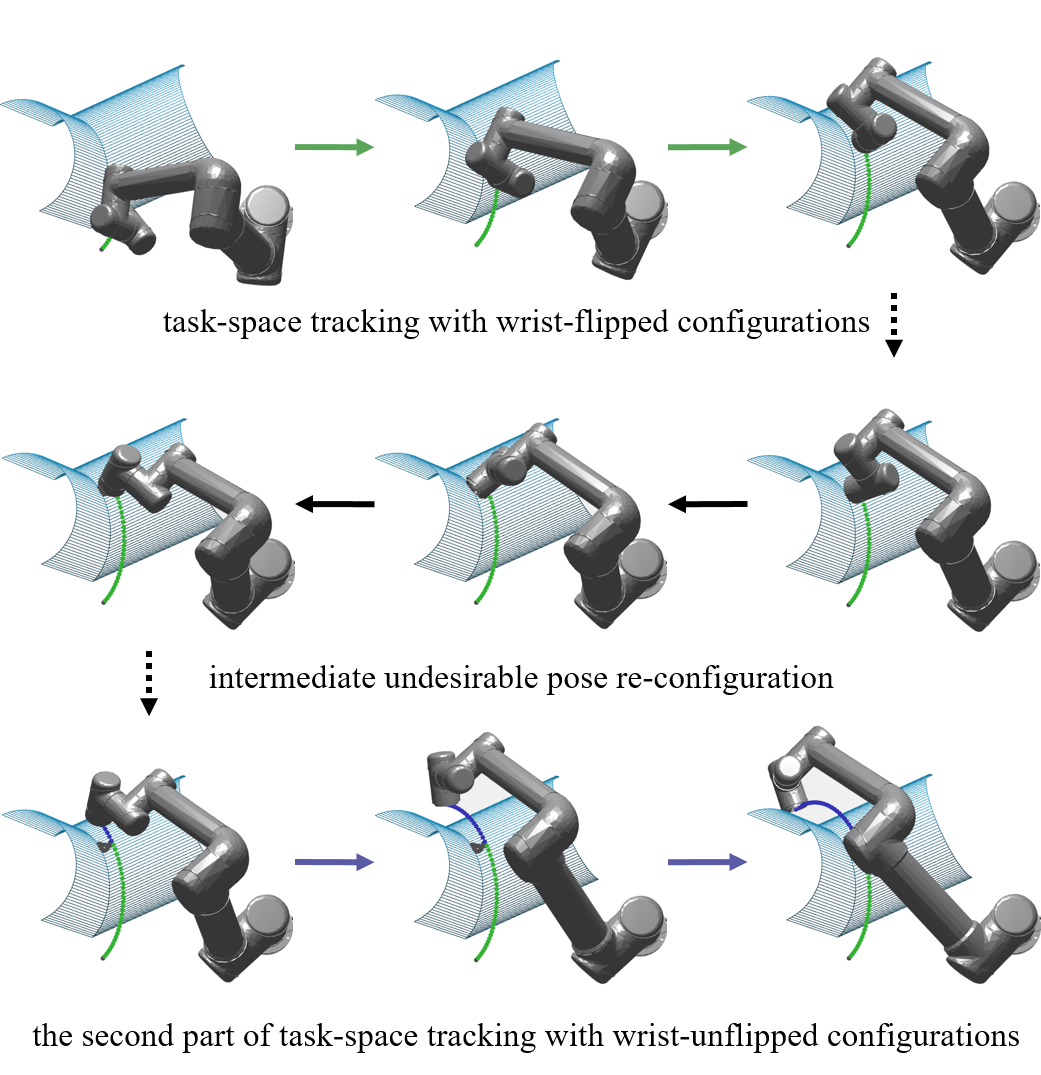
\includegraphics[width=0.48\textwidth]{figures/fig1/fig1_2}\label{fig:zerosolution}
\caption{Illustration of a welding task using a non-redundant manipulator. The intersecting curve of two cylinders, as well as the EE pose during the task is assumed well-defined. 
At the end of the first segment of continuous tracking (depicted in green), the wrist would hit the forearm if the manipulator moved further along the path. thus, in order to continue tracking the desired path, the manipulator must adopt a different configuration pose, in this case the wrist-unflipped pose is shown for illustration.}
\label{fig:demo1}
\end{figure}


An illustration of the TNTP problem applied to a figurative welding task is depicted in Fig.~\ref{fig:demo1}. Let the task-space path be the intersected curve between the two cylinders. 
To trace the path section closer to the manipulator base (EE path shown in green), the manipulator adopts the wrist-flipped configurations. 
However, there is limited reachability for the manipulator under this configuration in the far side of the path (EE tracking shown in blue in the bottom row, traversed later), as such the manipulator must readjust its pose and chooses to adopt a wrist-unflipped configuration. During the rearrangement, an undesirable motion of the EE path (shown in black) is introduced, together with the inevitable suspension of the path tracking at the point of take-off and re-landing. 
Finally, the manipulator is able to finish the tracking of the desired path with one pose reconfiguration (the latter part of EE tracking is depicted in blue). 

A key observation in this setting is the natural discontinuity between different inverse kinematics (IK) solutions of the same EE pose when discarding singular configurations: between an 
elbow-up configuration and an elbow-down configuration there must be a transition through a singular elbow-straight configuration, the neighbourhood of which is generally 
disregarded during planning~\cite{Mayorga1988Singularities}, particularly in industrial settings given a manipulator's controller ability to deal effectively with perturbations along singular dimensions~\cite{Xu2015Singularity}. 
As such, only the pairwise connectedness of valid IK solutions for consecutive EE waypoints needs consideration, and the problem of minimising the number of manipulator 
reconfigurations can be transformed into an efficient model to selecting connected pairs of IK solutions (as will be described in further detail in Section~\ref{section:modelling}.) 

In this paper, we discuss the optimal solution to the TNTP of non-redundant manipulators. Optimality in this context translates to the minimum number of EE deviations from the pre-defined path. The problem constitutes a generalisation of the classic task-space tracking problem seeking a joint-space continuous trajectory, essentially a zero-reconfiguration solution to the TNTP, if it exists. Whilst for the cases where no zero-reconfiguration solution prevails, the assignment can be regarded as ``failed" by existing (sampling) algorithms. However, the outcome via the proposed TNTP optimal scheme can now guarantee a solvable min-reconfiguration solution regardless. The contributions of this paper can be summarised as: 
\begin{enumerate}
\item A generalisation of the manipulator task-space tracking task into a TNTP with minimum reconfigurations, which is shown solvable. 
\item A computationally tractable solver. % <JVM> efficient or real-time? not sure we can claim that with the current data shown in the manuscrip
\item The open-sourcing~\footnote{An opensource implementation is provided here: \url{https://github.com/ZJUTongYang/min_reconfig_taskspace_tracking}} of the algorithm.
\end{enumerate}


\begin{figure}[t]
\centering
\subfigure[]{
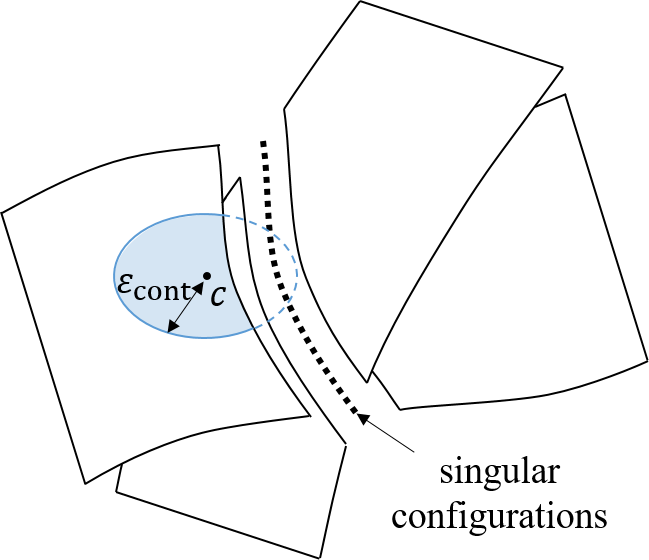
\includegraphics[width=0.21\textwidth]{figures/sing_a_2}\label{fig:sing:a}
}
\subfigure[]{
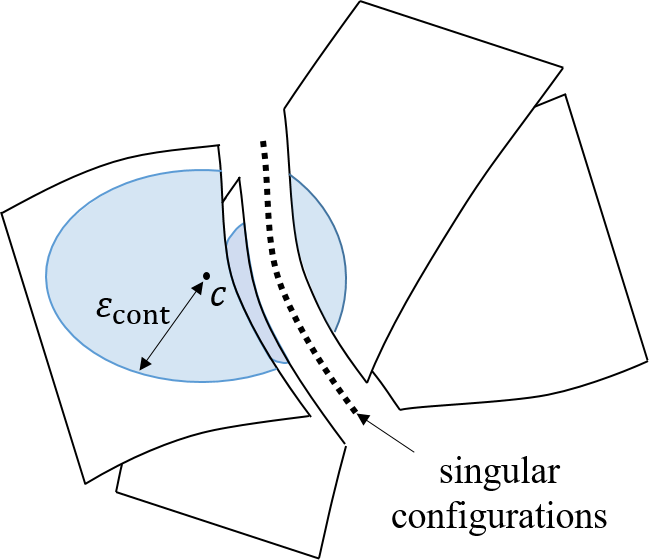
\includegraphics[width=0.21\textwidth]{figures/sing_b_2}\label{fig:sing:b}
}
\caption{Demonstration of the joint-space structure near singularities. The adoption of a manipulability measure implicitly forms a gap between disjointed sets of non-singular configurations. (a) A suitable choice of joint-space connectivity measure $\epsilon_{\rm cont}$ will provide correct judgment of connectedness between configurations (b) An unsuitable choice of $\epsilon_{\rm cont}$, where configurations from different sets might be mistakenly regarded as continuous. }\label{fig:sing}
\end{figure}



The remainder of this paper is organised as follows~\footnote{A video illustrating the concepts hereby described can be found here: \url{https://github.com/ZJUTongYang/min_reconfig_taskspace_tracking_video}} 
Section~\ref{section:related_work} reviews and contextualised the problem within the existing literature. 
Section~\ref{section:modelling} shows that the optimal non-redundant TNTP solution can be transformed into an optimal assignment of joint-space IK solutions. 
Section~\ref{section:solution} proposes a solver of the non-redundant TNTP, including a detailed algorithmic diagram, guaranteeing completeness and the uncovering of all the optimal solutions. % of the algorithm execution. 
Experimental results from simulations and on an actual non-redundant manipulator are collected in Section~\ref{section:experiments}, with final concluding remarks gathered in Section~\ref{section:conclusion}.  



\section{Related Work}\label{section:related_work}
The task-space tracking problem of a robot manipulator is %a decades-old research topics. 
an established research topic in the literature. Given a task-space path, the valid non-singular manipulator inverse kinematic (IK) solutions~\cite{Lavalle2006Planning} have been observed to form constrained subsets of the manipulator joint-space. 
When the manipulator transits between disjointed sets, the joint-space trajectory connecting configurations from disjointed sets will transition through at a singular state, in all likelihood making the end-effector veer off the pre-defined path, thus incurring an undesirable~\textit{ pose reconfiguration}.
%When the manipulator transits between disjointed sets, the joint-space trajectory connecting the configurations from disjointed sets is either singular or making the end-effector off the pre-defined path, which is referred to as the \textit{undesirable pose reconfiguration}. 

Existing algorithms focus on a local trajectory generation for task-space tracking, i.e., given the manipulator's current configuration with the EE docked on the pre-defined path at a given orientation, generate a control strategy for each manipulator joint such that the EE moves along the path. 
Redundancy of the manipulator has generally been assumed~\cite{Egeland1987Task} so that there exists an ample set of joint-space continuous configurations for continuous task-space tracking, among which valid singular configurations also exist to bridge non-singular configurations~\cite{Porta2012Randomized}. 
Since the algorithms only need to locally generate an instant motion, they are  more effeectively referred to as ``task-space controllers''~\cite{Xian2004Task}. 
When no local continuous tracking motion can be found, a joint-space path planner will be adopted to find an unrestricted motion towards a configuration ensuring the EE visiting the next task-space point. 

However, the structure of valid IK configurations becomes further scattered when the manipulator is non-redundant~\cite{Mayorga1987Singularities}, with obstacles in the environment compounding this condition~\cite{Khatib1986Real}, since each connected set of valid IK solutions has only the same dimension as its task-space preimage (e.g., a curve in 6D space as is the case here). Furthermore, no valid singularity exists for possible utilisation: a non-redundant manipulators in a singular state means it has lost the ability to dispense with perturbations imposed on the EE. As a result, a relatively sizeable task-space path is unlikely to find a continuous joint-space trajectory via traditional task-space controllers, and the manipulator will have to resort to adopting frequent pose reconfigurations during tracking. %A reduction in the number of reconfigurations to the minimum becomes crucial. This is to be presented in this work. 

More recent existing works~\cite{Yang2020Cellular}~\cite{Yang2020Nonrevisiting} have proposed cellular decomposition and graph theory
%shared the similar perspective to this work 
in solving the optimal surface coverage task, also explicitly considering the joint-space connectivity of IK solutions to visit different task-space points. 
%Note however that the solvers in~\cite{Yang2020Cellular}~\cite{Yang2020Nonrevisiting} are for surface coverage and are obviously exponential. 
The nature of the surface cell data makes these proposed solvers exponential. 
In contrast, the work proposed in this manuscript focuses on the more persistent tracking problem, where the computational efficiency for possible real-time applications needs to be carefully considered. Given the reduced dimensionality of the problem, a dynamic programming (DP) approach with an efficient greedy strategy can thus be adapted to reveal a globally optimal and complete solution. 


\section{Problem Modelling}\label{section:modelling}
In this section, the non-redundant manipulator TNTP is modelled. The commonly adoted ``planning-controlling" scheme is adopted to tackle the problem. During the planning stage, 
and subject to a given task-space path, a joint-space collision-free path is constructed, where consecutive configurations are ``close" enough such that their connectedness can be guaranteed. 
Subsequently, during the control stage, joint-space waypoints are interpolated and assigned suitable reaching times and joint velocities. 
The focus on this work is on the planning stage, where the manipulator IK relation is not one-to-one but one-to-many~\cite{Lavalle2006Planning}. % <JVM> add a red quickly if you read this
As such, selecting one from all valid IK solutions for each task-space waypoint becomes the fundamental problem. And the objective is doing it in way that reconfigurations are minimised, and guaranted at the planning stage. 
The discussion about control is assumed and outside the scope of the work. 



\subsection{Task-Space Discretisation and Valid Manipulator States}
Let the non-redundant TNTP problem be discussed in the ordinary 3D tracking scenario, where the manipulator is 6 DoF. 
The task-space path to be tracked is parameterised by a function curve $\gamma(t), t\in [0, 1]$ where each point $\gamma(t)$ is a 3D pose of the manipulator EE. 
If there are multiple intermediate stations for the EE to visit in order, we use a cubic interpolation to generate a continuous curve. 
Then, a suitable number (say $N$) of points are sampled from the curve, and we get a series of 3D EE poses $\gamma_i = \gamma(\frac{i-1}{N-1}), 1\leq i\leq N$. 
For each point $\gamma_i$, knowing the manipulator kinematics, the manipulability constraints~\cite{yoshikawa1990translational}, and the obstacles in the surrounding environment, a set of valid IK solutions are collected, denoted by $\{c(i, a_i)\}_{1\leq a_i\leq A_i}$ where $A_i$ denotes the number of valid IK solutions for visiting point $\gamma_i$. 
The manipulability constraint filters all singularities, which also excludes a neighbouring set of nonsingular configurations of the singularities and thus forms a non-zero width gap between disjointed sets of non-singular configurations. 
See Fig.~\ref{fig:sing} for an illustration.
If two non-singular configurations are joint-space connectable only by visiting singularities, as long as we set a small distance measure $\epsilon_{\rm cont}$ as shown in Fig.~\ref{fig:sing:a}, they will not be mistakenly regarded as connectable configurations. 
However, note that the width of the gap is implicit, so there does not exist an explicit formula for $\epsilon_{\rm cont}$. How to choose a suitable $\epsilon_{\rm cont}$ is to be presented in the next paragraph. 


For each valid manipulator configuration $c(i, a_i)$ we assign a state $D(i, a_i)$ as follows: 
For the first EE pose $\gamma_1$, let $\{D(1, a_1)\}_{1\leq a_1\leq A_1}$ be distinct numbers, such as $1, \cdots, A_1$. 
For the $i$-th ($2\leq i\leq N$) EE pose, we match $\{c(i, a_i)\}_{1\leq a_i\leq A_i}$ to the IK solutions of previous point $\{c(i-1, a_{i-1})\}_{1\leq a_{i-1}\leq A_{i-1}}$ whose state $\{D(i-1, a_{i-1})\}_{1\leq a_{i-1}\leq A_{i-1}}$ have been assigned. 
\begin{enumerate}
\item If $c(i, a_i)$ is joint-space continuous to a previous configuration $c(i-1, a_{i-1})$, then $D(i, a_i) = D(i-1, a_{i-1})$.
\item If $c(i, a_i)$ is not connectable to any configuration in $\{c(i-1, a_{i-1})\}_{1\leq a_{i-1}\leq A_{i-1}}$,  $D(i, a_i)$ is assigned a new state different from all existing states. 
\item If $c(i, a_i)$ is connectable to multiple IK solutions of the previous point, this indicates that different IK solutions of the same task-space pose are connectable without visiting singularities. This is a wrong judgment because of inappropriate waypoints selection and a too coarse joint-space connectivity measure. See Fig.~\ref{fig:sing:b} for an illustration. Then the task-space should be re-sampled with a higher resolution, the connectivity measure should be set smaller, and all above-mentioned processes need to be re-done. 
\end{enumerate}


\subsection{The Task-space Non-Revisiting Problem (TNTP)}

After all configurations are assigned a state, each task-space point has a set of possible states, $D(i)\triangleq \{D(i, a_i)\}_{1\leq a_i\leq A_i}$. 
Note that here we have assumed the non-nullity of $D(i)$, as if a task-space point is unreachable by any manipulator configuration, the TNTP problem is essentially divided into two sub-TNTP problem with the truncated task-space path segments. 
So the TNTP problem is finally transformed to the optimal design of state for each task-space point. 
A valid joint-space trajectory is a sequence of joint-space configurations, which can be represented by a vector of states,
\begin{equation}
S(j_1, j_2, \cdots, j_N) \triangleq [D(1, j_1), \cdots, D(N, j_N)],\ 1\leq j_i\leq A_i
\end{equation}
and the cost is defined by the number of switches of states, 
\begin{equation}\label{equ:cost}
g\left(S(j_1, \cdots, j_N)\right) \triangleq \sum\limits_{i = 1}^{N-1}\#\left\{D(i, j_i)\neq D(i+1, j_{i+1})\right\}
\end{equation}
The optimal solution to TNTP problem is to find all admissible sequences of configurations such that the cost is the globally minimum, 
\begin{equation}
\begin{aligned}
S^*(j_1, j_2, \cdots, j_N) = &\mathop{\rm argmin}\limits_{[j_1, \cdots, j_N]}~g(S(j_1, \cdots, j_N))\\
s.t.~~~~ &1\leq j_i\leq A_i,\ i = 1, \cdots, N
\end{aligned}
\end{equation}





%<ty> The algorithmic diagram is too long so we have to use [H] option. So we adjust the position of the diagram after we finish wording. 

\begin{algorithm}[H]
    \caption{Non-redundant TNTP Solver}\label{alg:1}
    \begin{algorithmic}[1]
        \Require Task-space path $\gamma$, obstacles in environment $\{O\}$, manipulator kinematics and collision model, manipulability constraint $\epsilon_{\rm sing}$, configuration connectedness measure $\epsilon_{\rm cont}$
        \Ensure All optimal joint-space trajectories 
\State //Select task-space points for IK calculation
\State $\{\gamma_i\}_{1\leq i\leq N} \leftarrow \gamma(\frac{i-1}{N-1}), 1\leq i \leq N$
\State //Calculate valid IK solutions for each point
\For{$1\leq i\leq N$}
\State $\{c(i, a_i)\}_{1\leq a_i\leq A_i}\leftarrow$ calculateValidIK($\gamma_i$)
\State $D(i, a_i) = -1, 1\leq a_i\leq A_i$
\EndFor
\State $\{D(i, a_i)\}_{\substack{1\leq i\leq N\\1\leq a_i\leq A_i}}\leftarrow $assignJointState($\{c(i, a_i)\}_{\substack{1\leq i\leq N\\1\leq a_i\leq A_i}}$)
\State $P =\{[0, \cdots, 0]\}, \tilde{P} = \varnothing$ // preserved solutions
\For{$1\leq i\leq N$}
\State //In the $i$-th stage
\For{each solution $S(a_1, \cdots, a_{i-1}, 0, \cdots, 0)$ in $P$}
\If{$\exists j_i, D(i, j_i) = D(i-1, a_{i-1})$}
\State // Greedy Strategy
\State create $p = S(a_1, \cdots, a_{i-1}, a_{i-1}, 0, \cdots, 0)$
\State push $p$ into $G(i, a_{i-1})$
\Else
\For{$1\leq j_i\leq A_i$}
\State create $p = S(a_1, \cdots, a_{i-1}, j_i, 0, \cdots, 0)$
\State push $p$ into $G(i, j_i)$
\EndFor
\EndIf
\EndFor
\For{$1\leq j_i\leq A_i$}
\State preserve only least-cost elements in $G(i, j_i)$
\State push $G(i, j_i)$ into $\tilde{P}$
\EndFor
\State $P \leftarrow \tilde{P}$
\EndFor
\State //All optimal solutions have been collected in $P$
\For{each element in $P$}
\State collect $\{c(i, a_i)\}_{1\leq i\leq N}$ based on $S(a_1, \cdots, a_N)$
\For{$1\leq i\leq N-1$}
\If{$c(i, a_i)$ and $c(i+1, a_{i+1})$ not continuous}
\State do bi-RRT from $c(i, a_i)$ to $c(i+1, a_{i+1})$ 
\State insert the undesirable motion between $c(i, a_i)$ and $c(i+1, a_{i+1})$
\EndIf
\EndFor
\EndFor
\State \Return $P$
    \end{algorithmic}  
\end{algorithm}

\begin{figure}[t]
\centering
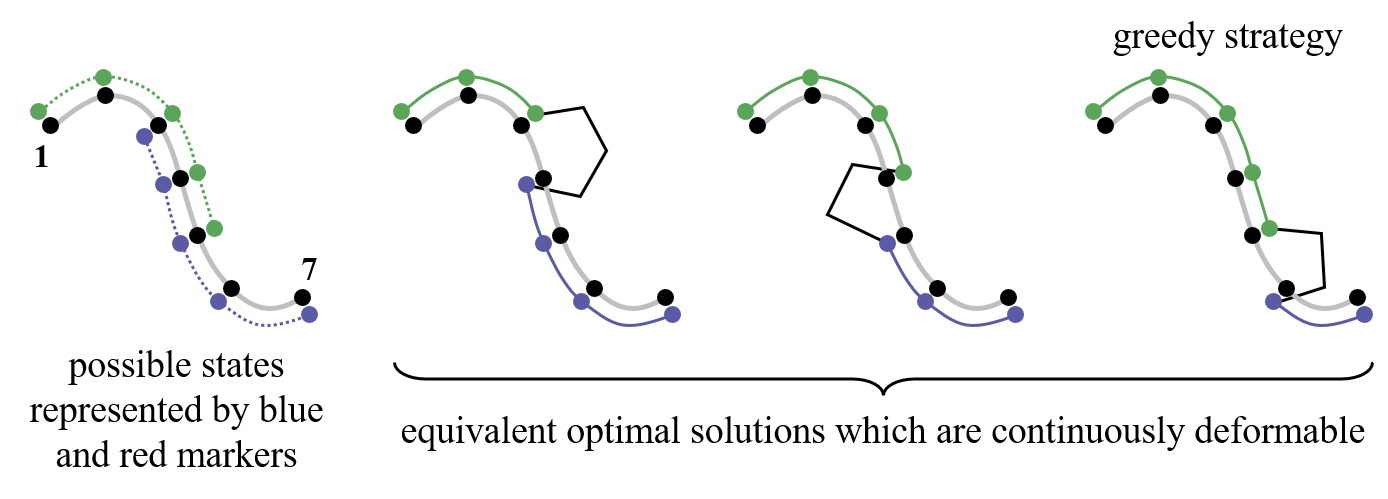
\includegraphics[width=0.48\textwidth]{figures/greedy}
\caption{Illustration of equivalent task-space tracking solutions. Given the $7$ discrete points sampled from a task-space curve, two sets of joint-space connected IK solutions are represented by green and blue dots. All solutions on the right consists of a continuous tracking motion with configurations represented by green, an undesirable motion denoted by black broken line, and a continuous tracking motion represented by blue, and they are all optimal solutions. The greedy strategy will find the last solution because it will lazily choose the configurations represented by green until it is not trackable. }\label{fig:equiv}
\end{figure}

\section{Optimal Solutions to TNTP}\label{section:solution}
In this section, the non-redundant TNTP problem is effectively solved, and all optimal solutions are proven collectable. 


\subsection{Principle of Optimality}

We observe that if the state of an intermediate point is assigned, then the calculation of cost becomes two independent parts. Denote the sub-TNTP problem in a similar form with less number of variables $n<N$, 
\begin{equation}
S(j_p, \cdots, j_q) \triangleq [D(p, j_p), \cdots, D(q, j_q)], 1\leq p <q \leq N
\end{equation}
with the cost defined similar as Eqn.~(\ref{equ:cost}). 
Let point $i$ be assigned with state $S(i, a_i)$, then 
\begin{equation}
\begin{aligned}
&\mathop{\rm argmin}\limits_{[j_1, \cdots, j_{i-1}, j_{i+1}, \cdots, j_N]} g(S(j_1, \cdots, j_{i-1}, a_i, j_{i+1}, \cdots, j_N))\\
&~~= \mathop{\rm argmin}\limits_{[j_1, \cdots, j_{i-1}]} g(S(j_1, \cdots, j_{i-1}, a_i))\\
&~~~~~~~~~~+\mathop{\rm argmin}\limits_{[j_{i+1}, \cdots, j_N]} g(S(a_i, j_{i+1}, \cdots, j_N))-1
\end{aligned}
\end{equation}
Here the last term $-1$ appears because when the manipulator finishes covering the last point of the first sub-TNTP with configuration $D(i, a_i)$, it has actually entered the second sub-TNTP with configuration $D(i, a_i)$ without EE lift-off. 
Then we can see that an optimal solution to the non-redundant TNTP must contain an optimal solution to the sub-TNTP, which essentially satisfies the principle of optimality for dynamic programming (DP)~\cite{Bellman2013Dynamic}. 
This motivates us to encode a partly-solved solution by the state of their frontier point:  
Let the state of points be assigned from point $1$ to point $N$, we denote the \textit{frontier point} by the last assigned point. 
We group the problem states with the same cost and the same decision on the frontier point, 
\begin{equation}
G(i, a_i) = \{S(j_1, \cdots, j_{i-1}, a_i)|1\leq j_k \leq A_k, 1\leq k\leq i-1\}
\end{equation}

In the first stage, all possible states of point $1$ are collected, with sets $G(1, 1), \cdots, G(1, A_1)$ being obviously constructed with only one element in each set. 
In the $i(\geq 2)$-th stage, the state of point $1\sim(i-1)$ has been assigned and different solutions are collected. After the state of point $i$ is assigned and the cost is updated, all solutions are re-grouped by the state of point $i$. Only the least-cost solutions are still preserved for the subsequent iteration. 

\begin{figure*}[t]
\centering
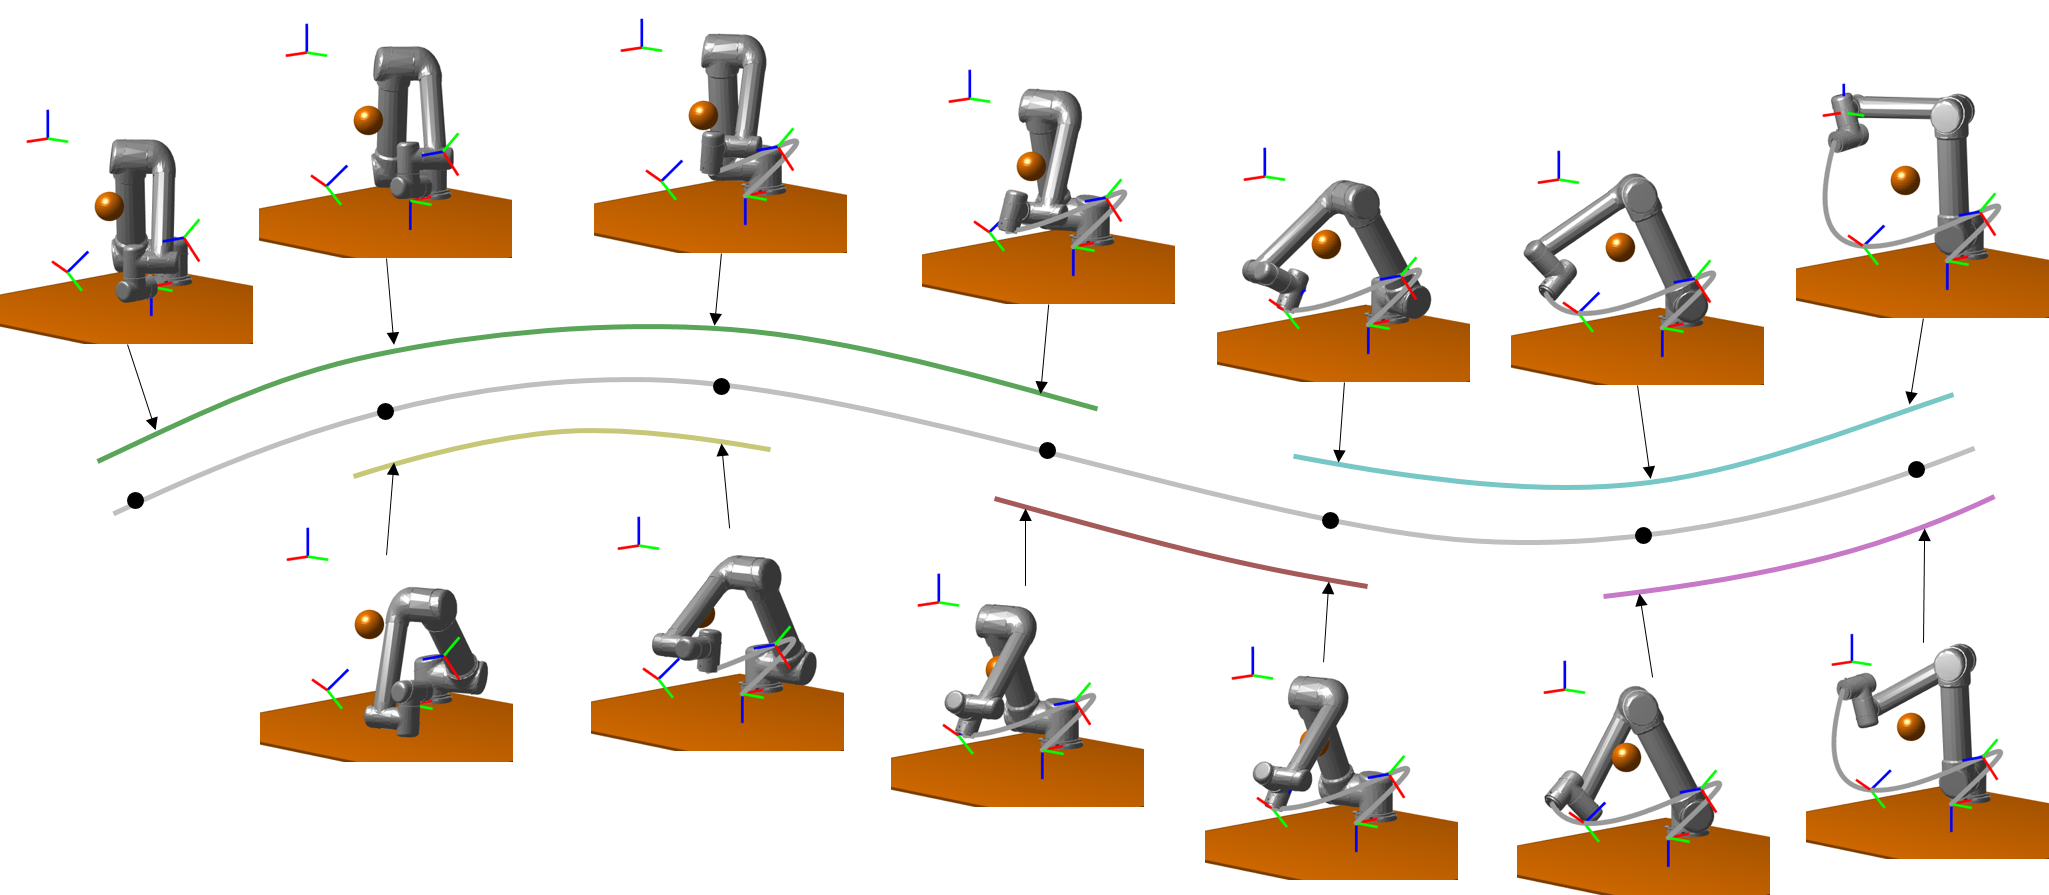
\includegraphics[width=0.96\textwidth]{figures/case_study/comb_3}
\caption{Illustration of valid IK solutions along the task-space path. 
The coloured curves show the joint-space connectivity between configurations. }\label{fig:allpose}
\end{figure*}

\subsection{Greedy Strategy}\label{section:greedy}
Generally, the greedy strategy performs much faster than the dynamic programming strategy since no back-tracking process is required. However, it might not guarantee the global optimality (minimum of cost). 
In this subsection we show that greedy choosing the continuous configurations preserves global optimality and completeness of collecting all optimal solutions. 
The global optimality is verified by observing that in the $i$-th stage, let there exist a state of point $i$ which is equal to $a_{i-1}$, 
\begin{equation}\label{equ:optimality}
\begin{aligned}
&\mathop{\rm argmin}\limits_{[j_i, \cdots, j_N]} g(S(a_1, \cdots, a_{i-1}, j_i, \cdots, j_N))\\
=&g(S(a_1, \cdots, a_{i-1})) - 1 + \mathop{\rm argmin}\limits_{[j_i, \cdots, j_N]} g(S(a_{i-1}, j_i, \cdots, j_N))\\
=&g(S(a_1, \cdots, a_{i-1})) - 1 \\
+& \left\{
\begin{aligned}
&\mathop{\rm argmin}\limits_{[j_{i+1}, \cdots, j_N]} g(S(a_{i-1}, a_{i-1}, j_{i+1}, \cdots, j_N))\\
&\mathop{\rm argmin}\limits_{[j_{i+1}, \cdots, j_N]} g(S(a_{i-1}, a_i, \cdots, j_N))+1, \mbox{ enforce }a_i\neq a_{i-1}
\end{aligned}\right.\\
=&g(S(a_1, \cdots, a_{i-1})) - 1 \\
+&\left\{
\begin{aligned}
	&\left\{
	\begin{aligned}
		&\mathop{\rm argmin}\limits_{[j_{i+2}, \cdots, j_N]} g(S(a_{i-1}, a_{i-1}, a_{i-1}, \cdots, j_N)), \mbox{ if } a_{i+1}=a_{i-1}\\
		&\mathop{\rm argmin}\limits_{[j_{i+2}, \cdots, j_N]} g(S(a_{i-1}, a_{i-1}, a_{i+1}, \cdots, j_N))+1, \mbox{ else }
	\end{aligned}
	\right.\\
	&\mathop{\rm argmin}\limits_{[j_{i+1}, \cdots, j_N]} g(S(a_{i-1}, a_i, \cdots, j_N))+1, \mbox{ enforce }a_i\neq a_{i-1}
\end{aligned}
\right.
\end{aligned}
\end{equation}
We can know that if we assign $j_i = a_{i-1}$, the cost will be always no higher than assigning other state $j_i\neq a_{i-1}$ to point $i$, no matter in the next stage whether point $(i+1)$ will have the same state as point $i$. 
Hence, when the next unassigned point has a same possible state as the frontier point, we can discard all other possible states and directly assign this one. 

Next, we show that no optimal solution is missed by the greedy choice of states. 
If the greedy strategy is not complete, that means an optimal solution contains one of the discarded states by the greedy selection of state, which will be proven retrievable by the collected optimal solutions. 
Continue the deduction in Eqn.~(\ref{equ:optimality}) we have 
\begin{equation}
\begin{aligned}
&\cdots (\mbox{Eqn.}~(\ref{equ:optimality}))\\
=&g(S(a_1, \cdots, a_{i-1})) - 1 \\
+&\left\{
\begin{aligned}
	&\left\{
	\begin{aligned}
		&\mathop{\rm argmin}\limits_{[j_{i+2}, \cdots, j_N]} g(S(a_{i-1}, a_{i-1}, a_{i-1}, \cdots, j_N)), \mbox{ if } a_{i+1}=a_{i-1}\\
		&{\color{blue}\mathop{\rm argmin}\limits_{[j_{i+2}, \cdots, j_N]} g(S(a_{i-1}, a_{i-1}, a_{i+1}, \cdots, j_N))+1, \mbox{ else }}
	\end{aligned}
	\right.\\
  &\left\{
	\begin{aligned}
		&\mathop{\rm argmin}\limits_{[j_{i+2}, \cdots, j_N]} g(S(a_{i-1}, a_i, a_i\cdots, j_N))+1, \mbox{ if }a_{i+1}= a_i\\
		&{\color{red}\mathop{\rm argmin}\limits_{[j_{i+2}, \cdots, j_N]} g(S(a_{i-1}, a_i, a_{i+1}, \cdots, j_N))+2, \mbox{ else }}
	\end{aligned}
	\right.
\end{aligned}
\right.
\end{aligned}
\end{equation}
Note that the term written in red has higher cost than the term written in blue, so a discarded state of the current point contributes to an optimal solution only when there exists a same state for the next point and the algorithm assigns it to the next point in the next stage. 
However, note that the solutions are obviously equivalent, as when a point can be continuously visited together with either its previous point or its subsequent point, the two solutions are both optimal and can continuously transform from one to another by locally adjusting the point for the EE to leave the task-space path.
See Fig.~\ref{fig:equiv} for an illustration. 
Hence, all optimal solutions are proven collectable by a  dynamic programming approach with greedy utilisation of continuous manipulator configurations. 





\section{Experiments}\label{section:experiments}
The proposed algorithm generates all optimal joint-space trajectories ensuring the task-space tracking of a given EE path and minimum number of manipulator pose reconfigurations. Simulated and real-world experiments are presented in this section. 
In section~\ref{section:case_study}, the detailed explanation about a case study is presented, with valid  manipulator IK configurations illustrated, showing the necessity of manipulator pose re-configuration. 
To the authors' knowledge, there has not been an efficient algorithm for task-space tracking when the manipulator cannot follow the pre-defined path, as such all discussions were taken for redundant manipulators. So in section~\ref{section:comparison} we compare the proposed algorithm with the commonly used approach of randomly selecting the next configuration when the continuous tracking is impossible.
In section~\ref{section:realworld}, the proposed algorithm is tested on a real-world Universal Robots UR5 manipulator. 
An opensource implementation in MATLAB is presented here: \url{https://github.com/ZJUTongYang/min_reconfig_taskspace_tracking}. 

\begin{figure}[t]
\centering
\subfigure[]{
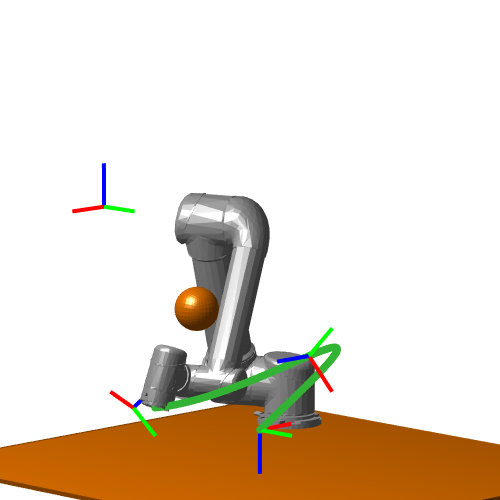
\includegraphics[width=0.14\textwidth]{figures/case_study/pose1_151}\label{fig:case_study:a}
}
\subfigure[]{
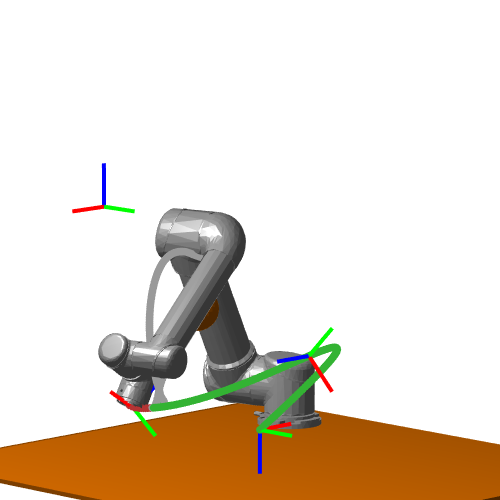
\includegraphics[width=0.14\textwidth]{figures/case_study/pose2_390}\label{fig:case_study:b}
}
\subfigure[]{
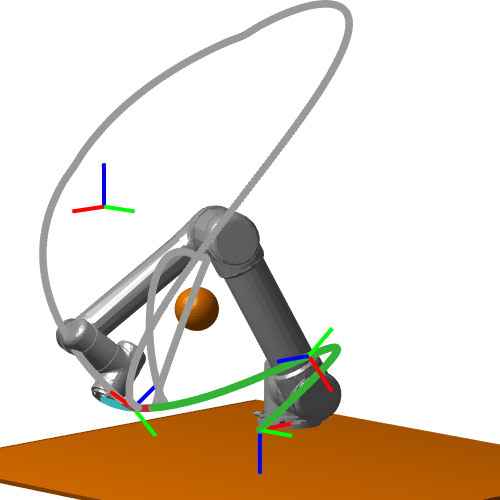
\includegraphics[width=0.14\textwidth]{figures/case_study/pose3_780}\label{fig:case_study:c}
}
\caption{Illustration of a task-space tracking where two manipulator reconfigurations are required. The three segments of continuous task-space tracking process (EE poses) are marked by green, red, and cyan colour in order. The gray curves show the trace of EE during manipulator reconfiguration. }\label{fig:case_study}
\end{figure}


\begin{figure}[t]
\centering
\subfigure[Case $1$]{
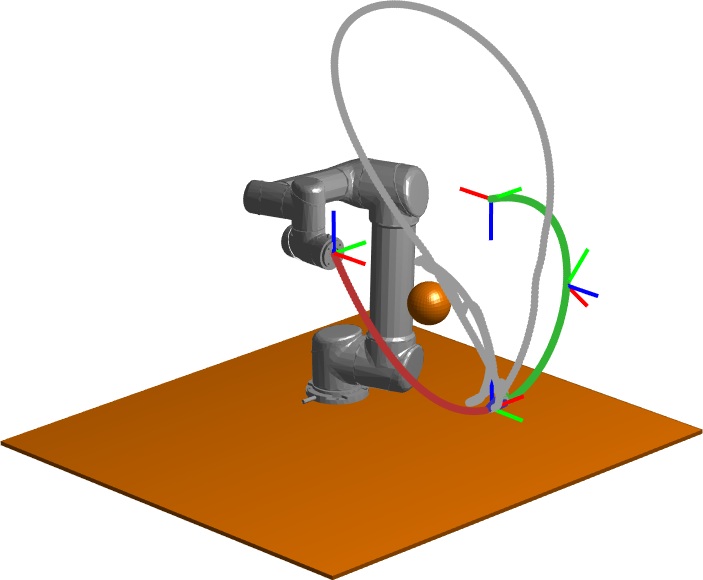
\includegraphics[width=0.24\textwidth]{figures/newcomparison/new_example_1_left}
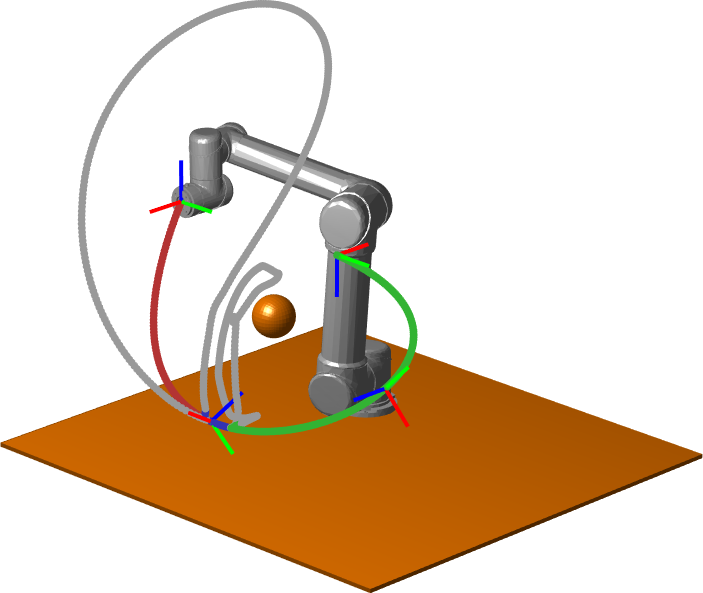
\includegraphics[width=0.24\textwidth]{figures/newcomparison/new_example_1_right}
}
\subfigure[Case $2$]{
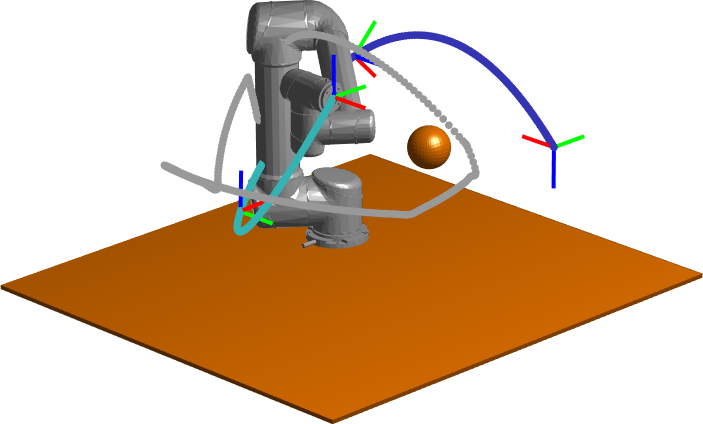
\includegraphics[width=0.24\textwidth]{figures/newcomparison/new_example_2_left}
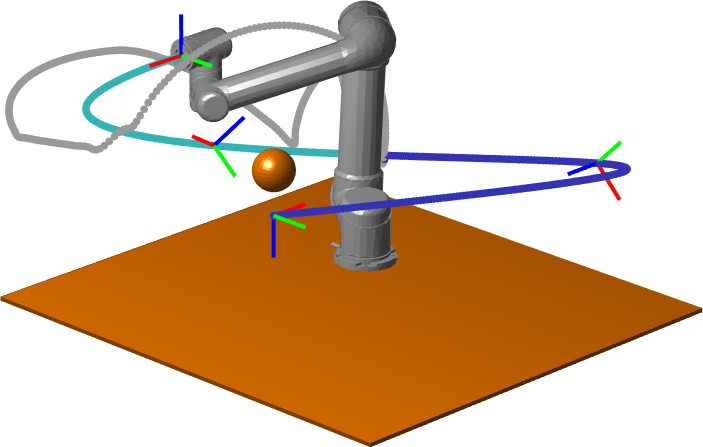
\includegraphics[width=0.24\textwidth]{figures/newcomparison/new_example_2_right}
}
\subfigure[Case $3$]{
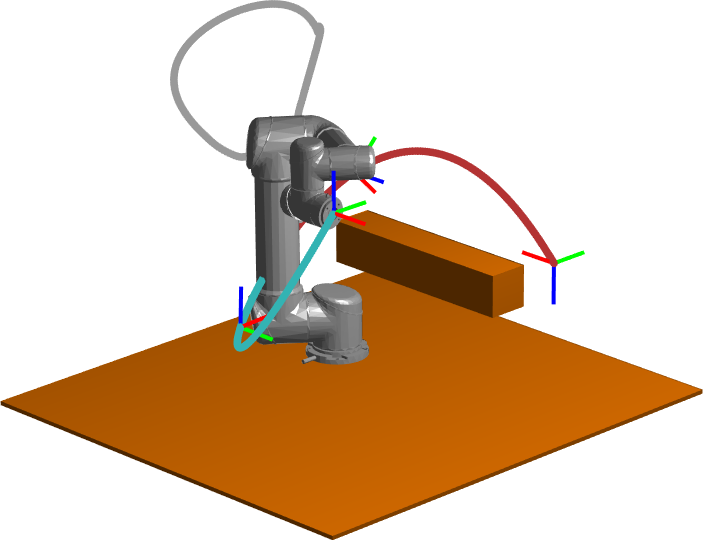
\includegraphics[width=0.24\textwidth]{figures/newcomparison/new_example_3_left}
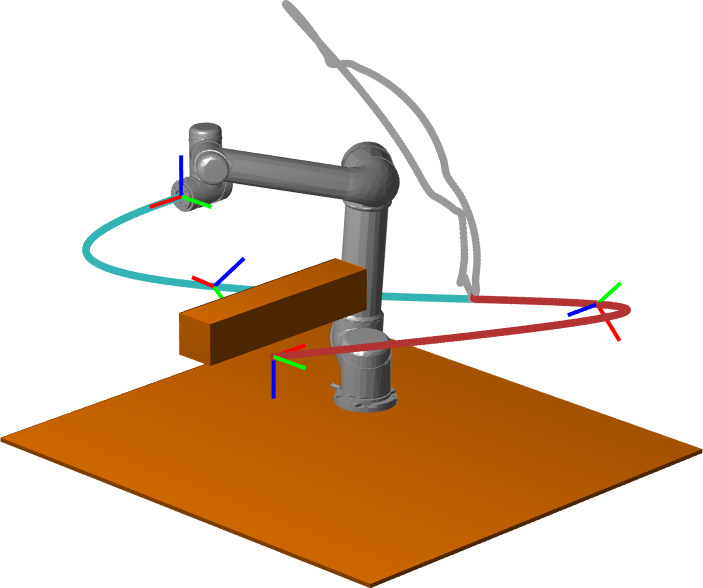
\includegraphics[width=0.24\textwidth]{figures/newcomparison/new_example_3_right}
}
\caption{Illustration of simulated comparison tests. The trajectories shown in figures are the optimal solutions generated by the proposed algorithm.}\label{fig:comparison}
\end{figure}

\subsection{Case Study}\label{section:case_study}


A task-space tracking process is shown here as a case study of the proposed algorithm. 
The task-space path is generated by interpolating four EE waypoints. 
Some valid IK solutions are collected in Fig.~\ref{fig:allpose} for better illustration of this case study. 
For one of the optimal tracking solution see Fig.~\ref{fig:case_study}. 
Obstacles in the environment are a ground plane and a sphere. 
Because the starting point of the task-space curve is near the ground, only one IK solution is valid (marked by green dots) so the manipulator would adopt it. 
However, after the manipulator is about to reach the third intermediate goal, the forearm will hit the spherical obstacle, so one pose reconfiguration is required. 
The last configuration of the first segment of tracking is shown in Fig.~\ref{fig:case_study:a}. 
By changing to a configuration like shown in Fig.~\ref{fig:case_study:b}, the forearm is lifted a little, above the wrist, which makes the EE visit the third intermediate goal. However, the forearm will still hit the spherical obstacle if it continues tracking, where another pose reconfiguration is required. 
See Fig.~\ref{fig:case_study:c}, by adjusting the configuration from shoulder-right to shoulder-left, the manipulator is able to finish the tracking task without colliding the spherical obstacle.
The reader is referred to our supplementary video to observe the full animation of this case study. 

%\begin{table}[t]
%\centering
%\caption{Simulation Results Versus Sampling-based Planners}\label{table:comparison}
%\begin{tabular}{c|c|c|c}
%\hline
%Case & Min-Reconfig(ours) & Mean-Reconfig& Probability\\
%\hline
%\hline
%case $1$ & $\mathbf{2}$ & $6.25$ & $1/256=0.39\%$\\
%\hline 
%case $2$ & $\mathbf{1}$ & $9.956$ & $5/6451\approx0.08\%$\\
%\hline
%case $3$ & $\mathbf{1}$ & $5.10$ & $1/90\approx 1.11\%$\\
%\hline
%\end{tabular}
%\end{table}



\begin{table}[t]
\centering
\caption{Simulation Results Versus Sampling-based Planners}\label{table:comparison}
\begin{tabular}{c|c|c|c|c}
\hline
Case & Min$^1$ & Time$^2$& Mean-Reconfig& Probability \\
\hline
\hline
case $1$ & $\mathbf{2}$ & 15ms & $6.25$ & $1/256=0.39\%$\\
\hline 
case $2$ & $\mathbf{1}$ & 9ms& $9.956$ & $5/6451\approx0.08\%$\\
\hline
case $3$ & $\mathbf{1}$ & 30ms& $5.10$ & $1/90\approx 1.11\%$\\
\hline
\end{tabular}
\begin{tablenotes}
\item $^1$ Ours
\item $^2$ Computational time is included simply for relative discrimination. Collision checking and detour planning during the undesirable motion are not included in the calculation. 
\end{tablenotes}
\end{table}

\begin{figure}[t]
\centering
\subfigure[]{
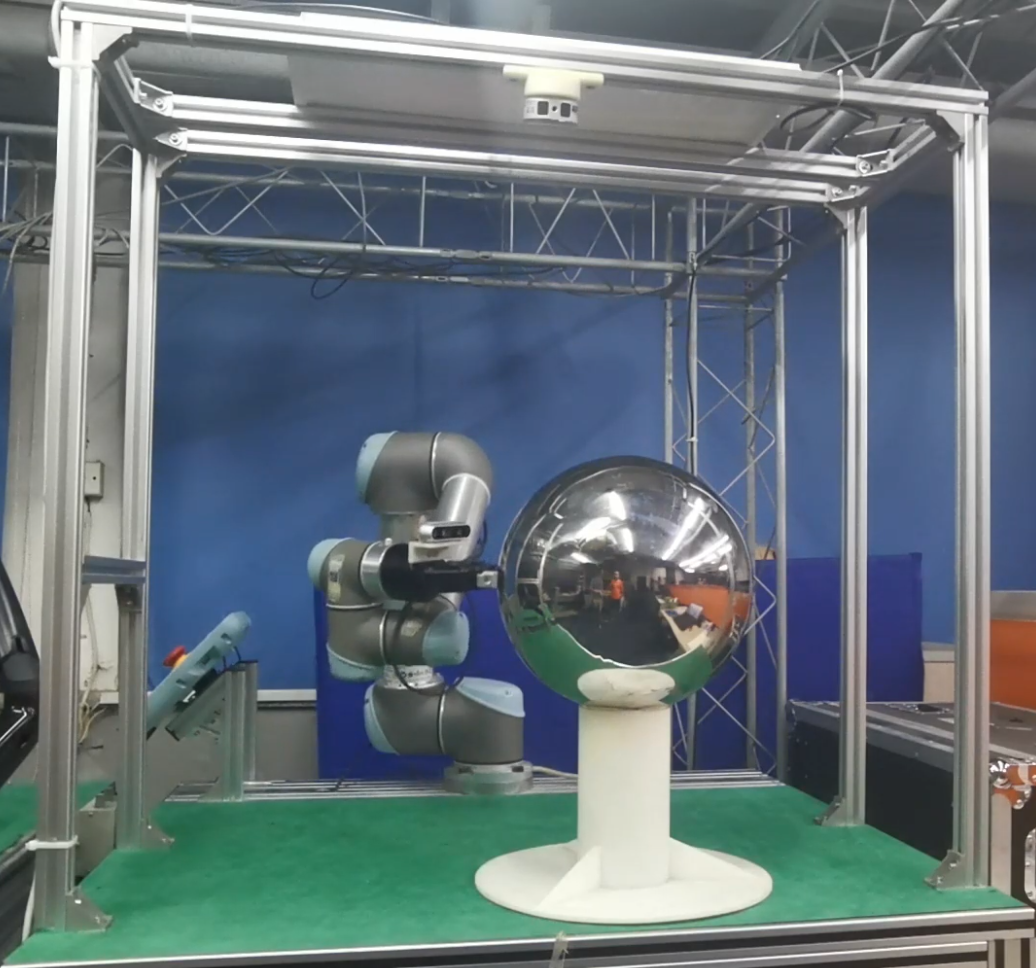
\includegraphics[width=0.22\textwidth]{figures/realworld/realworld_scenario}\label{fig:realworld_illustration:a}
}
\subfigure[]{
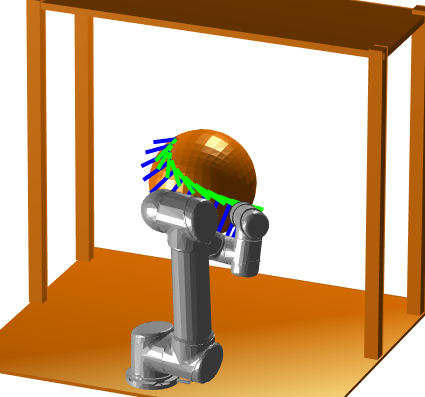
\includegraphics[width=0.22\textwidth]{figures/realworld/simulated_scenario_2}\label{fig:realworld_illustration:b}
}
\caption{The real-world scenario and its corresponding simulated environment. }\label{fig:realworld_illustration}
\end{figure}



\begin{figure*}[t]
\centering
\subfigure[]{
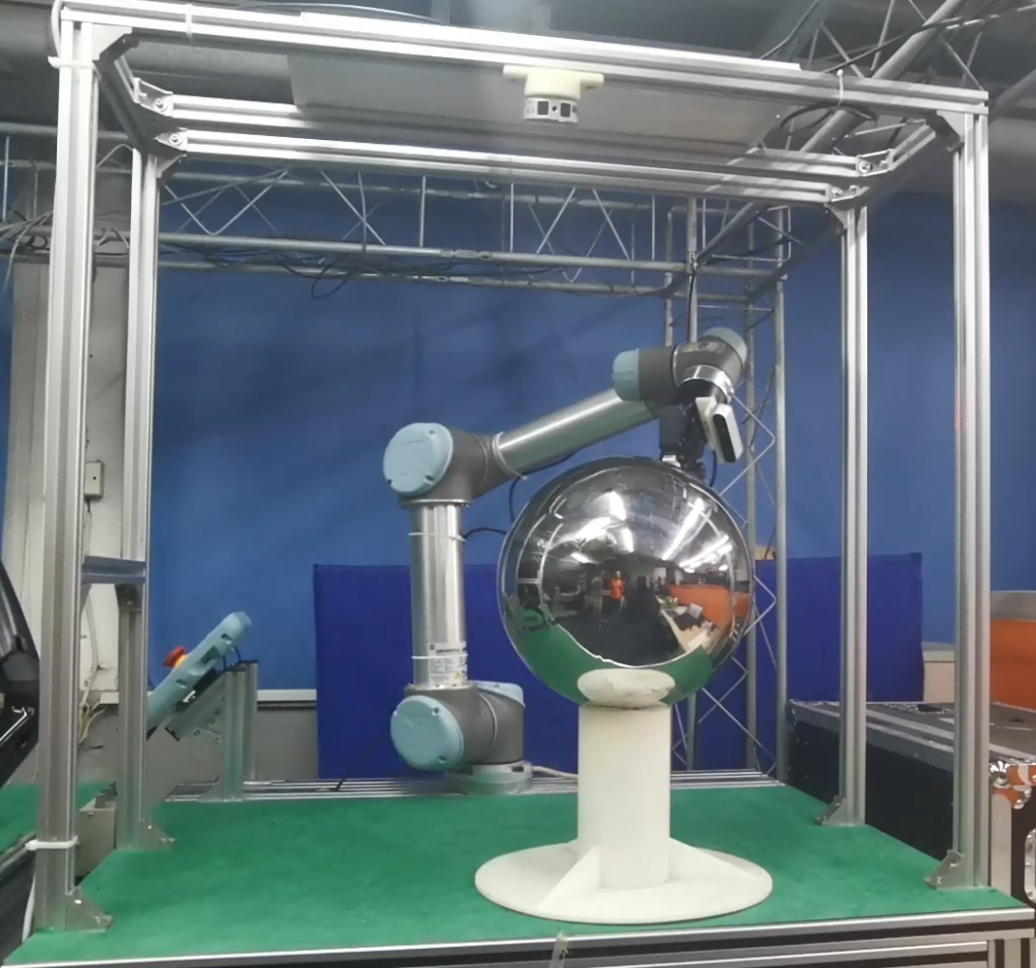
\includegraphics[width=0.18\textwidth]{figures/realworld/1}\label{fig:realworld_steps:a}
}
\subfigure[]{
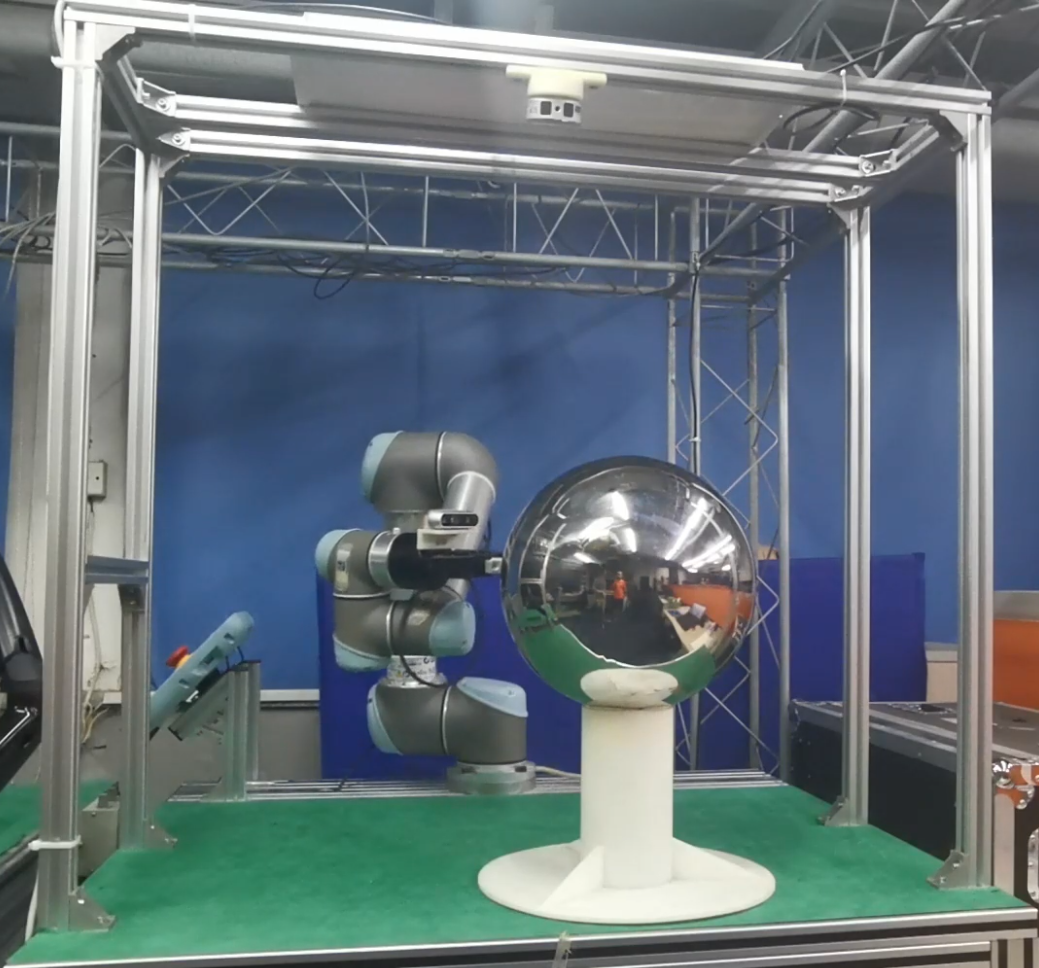
\includegraphics[width=0.18\textwidth]{figures/realworld/2}\label{fig:realworld_steps:b}
}
\subfigure[]{
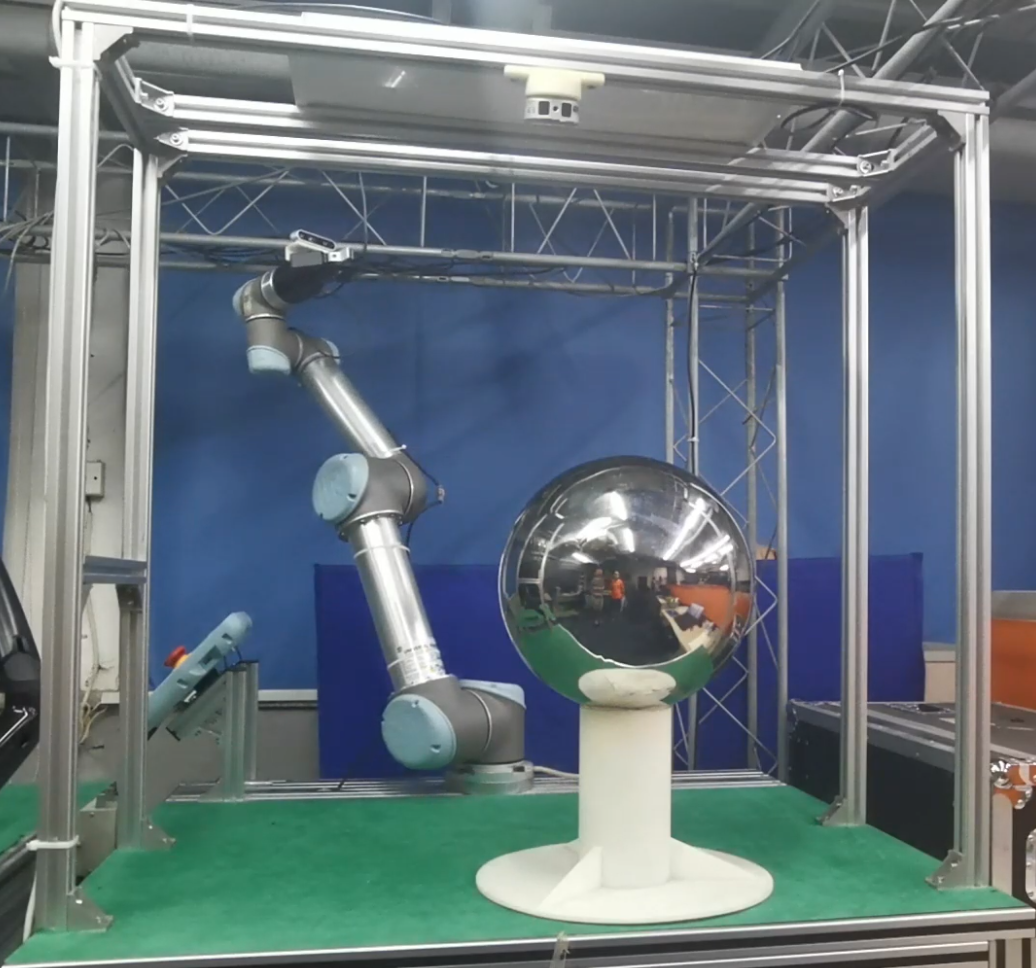
\includegraphics[width=0.18\textwidth]{figures/realworld/3}\label{fig:realworld_steps:c}
}
\subfigure[]{
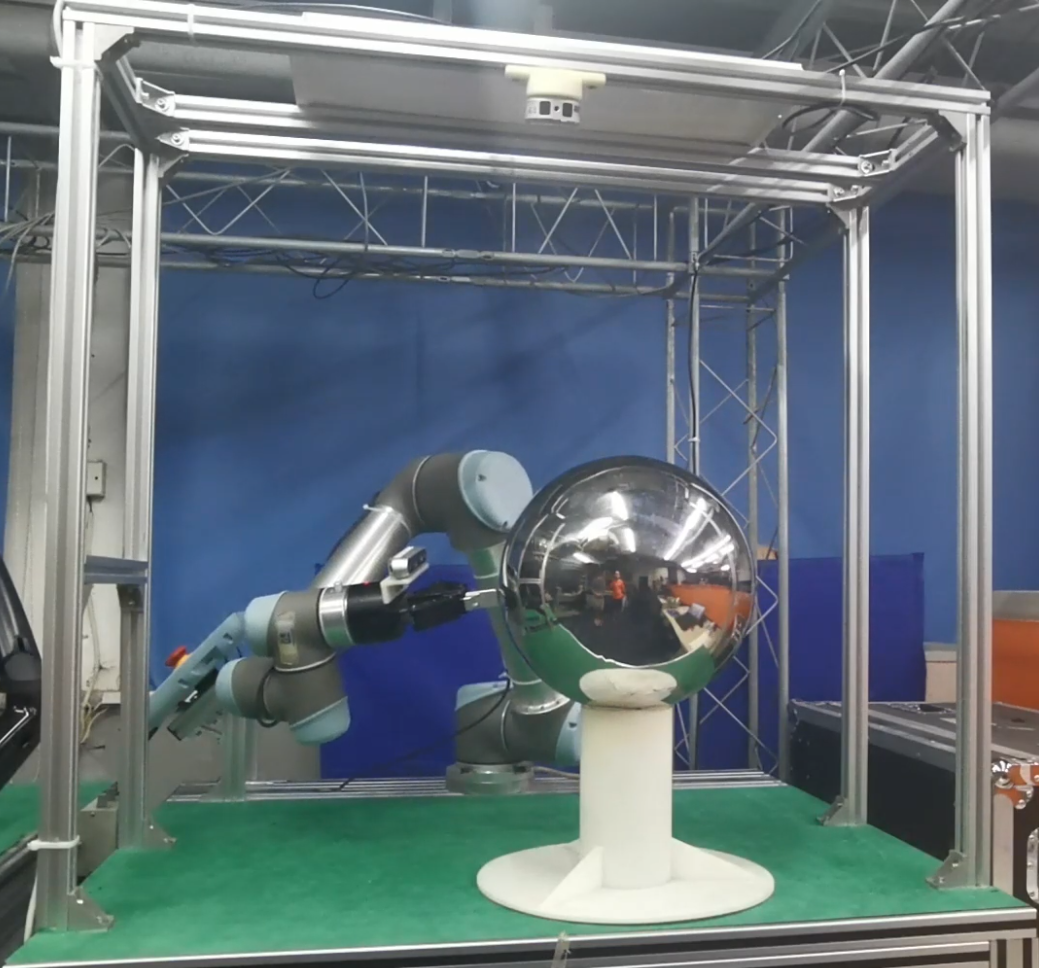
\includegraphics[width=0.18\textwidth]{figures/realworld/4}\label{fig:realworld_steps:d}
}
\subfigure[]{
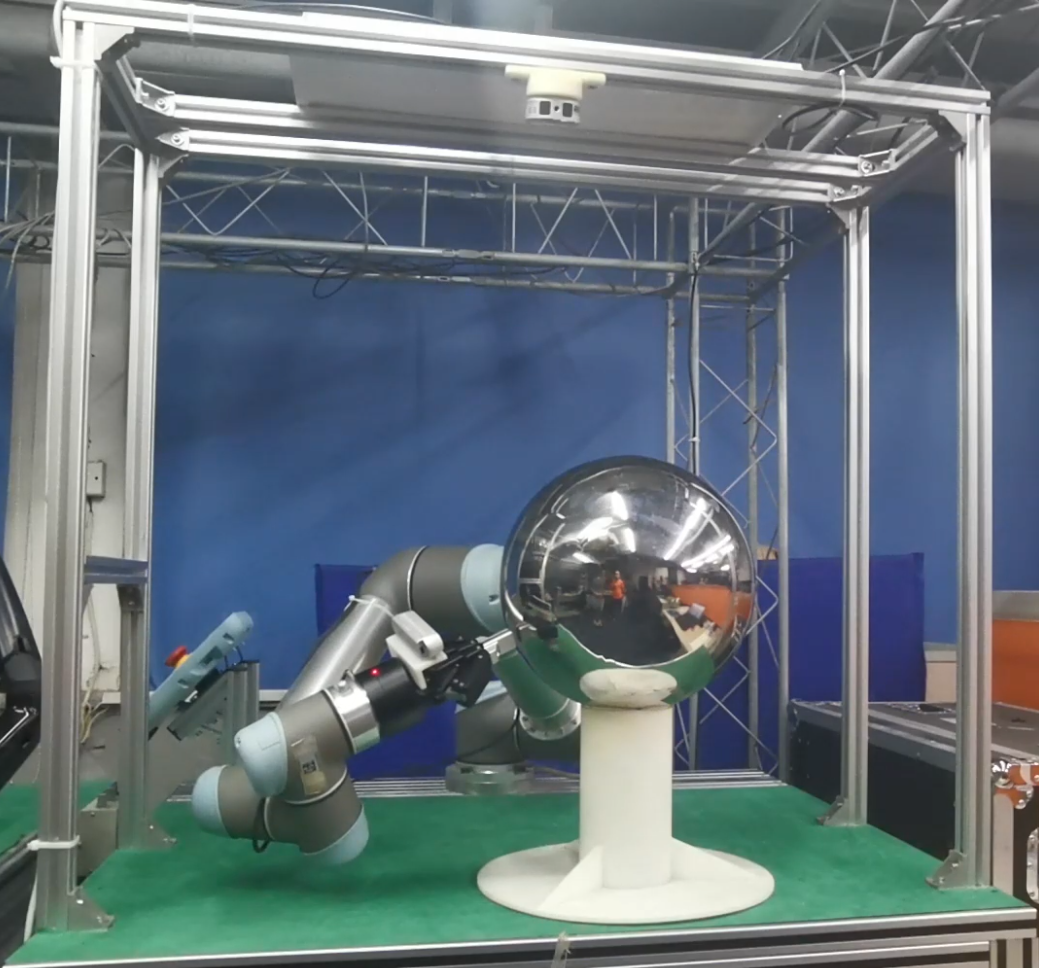
\includegraphics[width=0.18\textwidth]{figures/realworld/5}\label{fig:realworld_steps:e}
}
\caption{Illustrations of the manipulator configurations for the real-world tests. }\label{fig:realworld_steps}
\end{figure*}

\subsection{Comparison with  Sampling-based Planners}\label{section:comparison}
All existing solvers for task-space tracking are locally calculating a joint-space admissible trajectory, and when there is locally no valid trajectory to continue tracking, a joint-space path planner (such as the RRT~\cite{Lavalle2006Planning} used in this work, as often employed in mannipulator planning software such as the widely used  MoveIt!~\footnote{\url{https://moveit.ros.org/}} by the ROS research community, % <JVM> ref or www
and the OPML~\footnote{\url{http://ompl.kavrakilab.org/}} % <JVM> also
it is based on underneath) is carried out, as such the selected IK solution for visiting the next task-space point is randomly chosen. 
For fair evaluation, we assume the random selection of the IK solution for visiting the first task-space point, and the algorithms will greedily choose the continuous IK solutions. 
When the manipulator has to perform a pose reconfiguration motion, the starting pose of the next segment of task-space tracking is again randomly assigned. 

An illustration of thel tested cases is shown in Fig.~\ref{fig:comparison}, whilst some relevant statistics for comparison of the  different cases are collected in Table~\ref{table:comparison}. 
``Min-Reconfig"  refers to the minimum number of necessary manipulator pose reconfigurations generated by the proposed algorithm. 
For a fair evaluation of the performance of sampling-based planners in these settings, all possible assignments of IK configurations are enumerated, and the mean number of pose reconfigurations for all possible situations collected as ``Mean-Reconfig". 
The last column ``Probability" is the proportion of ``all optimal solutions / all possible solutions", which shows the probability of a sampling-based planner in coincidently obtaining a globally optimal solution. 
For example, in case $1$, there are $256$ different greedy assignments for the segments of continuous task-space motion, among which only one solution identifies with the optimal solution (with 2 reconfigurations). The average number of pose reconfigurations is shown to be $6.25$. The reader is referred to the supplementary video for further visualisations and comparatives during the resulting planning motions. 

Note that it is not the focus of this work to exhaustively compare the performance of different joint-space planners that may be able to produce marginally better reconfiguration trajectory in relation EE lift-off and task space continuity. It is apparent that without a mechanism to select a globally optimal IK solution to visit at the next iteration along the path, solutions based on traditoinal sampling-based planners 
will inevitably lead to unnecessary manipulator reconfigurations regardless. In fact the examples in this work have shown a nearly $99\%$ certainty to obtain a non-optimal choice with traditional planners ( $1 - \mbox{Prob.}$ in the last colum in Table~\ref{table:comparison}).
%will almost surely ($\approx 99\%$)lead to unnecessary manipulator reconfigurations regardless. 
% almost surely ($\approx 99\%$) obtain a non-optimal choice, 
%will inevitably lead to unnecessary manipulator reconfigurations regardless. 




\subsection{Real-world Illustration}\label{section:realworld}
The proposed algorithm is also evaluated in a real-world scenario. 
The real-world environment is modelled into MATLAB as shown in Fig.~\ref{fig:realworld_illustration}. Let the task-space path be a surface curve on the sphere. 
The $x$-axis of the EE is parallel to the surface normal vector, and the $y$-axis is parallel to the tangent of the surface curve, then $z$-axis is well-defined following the right-hand coordinates. As such the task is non-redundant for a $6$-Dof manipulator. The gripper imitates a non-zero length tool whose collision model is set as a cylinder (visualisation omitted in Fig.~\ref{fig:realworld_illustration:b}). 

See Fig.~\ref{fig:realworld_steps} for illustration. To pursue the optimal solution, the manipulator is instructed by the proposed algorithm to start tracking with the configuration as Fig.~\ref{fig:realworld_steps:a}, as such the manipulator can continuously track the task-space path until the pose in Fig.~\ref{fig:realworld_steps:b}, where the wrist is about to hit the forearm. 
One pose reconfiguration from a shoulder-right configuration (Fig.~\ref{fig:realworld_steps:b}) to a shoulder-left configuration (Fig.~\ref{fig:realworld_steps:d}) becomes necessary, between which an undesirable motion exists (Fig.~\ref{fig:realworld_steps:c}). It can be easily observed from our supplementary video how the undesirable motion calls for a large workcell and be time/energy inefficient. Finally, the manipulator is able to finish the task-space tracking with only $1$ (optimal) pose reconfiguration. 

\section{Conclusion}\label{section:conclusion}
A novel mechanism to generate an optimal joint-space trajectory for the task-space nonrevisiting tracking problem (TNTP) has been proposed in this work. 
The optimality is translated to the minimum number of segmentations of the pre-defined path caused by nonlinear manipulator kinematics and collision with obstacles in the environment. 
Manipulator reconfigurations are shown to be necessary for concatenating consecutive segments of continuous task-space tracking. These undesirable deviations result in additional time and energy penalties.
When compared to existing task-space tracking solutions, the proposed algorithm provides a globally optimal perspective to the choice of suitable manipulator inverse kinematics, 
maximising the joint-space connectedness during the tracking task. 
All optimal solutions (sequences of IK solutions ensuring mininmal reconfigurations) are proven collected via a dynamic programming solver, where a proposed greedy speeding-up strategy is shown to be without loss of global optimality and completeness. 
Simulated comparisons and real-world illustration has proven the validity of the proposed algorithm, with substantial reconfigurability improvements. 
These have been supplemented by a detailed video and an open sources implementation of the MATLAB implementation for the benefit of the research community. 

On a side note, or perhaps for future work embedded in other work, we argue that the proposed algorithm calculates a ``joint-space" cost of a task-space path. 
A metric based on the simple summation of joint-space distance between consecutive valid IK configurations is not an appropriate measure of cost, as manipulator reconfigurations significantly influence the performance of tracking and cannot be overlooked. 
In contrast, the proposed algorithm, with a minimum number of manipulator reconfigurations being explicitly considered, builds a more realistic estimation of the task-space tracking cost, which might be inspirational to the community. 







%The proposed scheme thus provides two relevant contributions to the map building problem
%\addtolength{\textheight}{-12cm}   % This command serves to balance the column lengths

%%%%%%%%%%%%%%%%%%%%%%%%%%%%%%%%%%%%%%%%%%%%%%%%%%%%%%%%%%%%%%%%%%%%%%%%%%%%%%%%

\bibliographystyle{ieeetr} %% setting the cite style
\bibliography{RAL22}

\newpage



\end{document}
